\chapter{Case study: Monitoring and control of air quality}

\label{chap:case-staudyAC}
This chapter presents a case study that joins the aggregate computing paradigm and a LoRaWAN network. Finally, it shows a simulation of the case study in the DingNet simulator.

\section{Case study description}
Nowadays air pollution is a very common problem of cities of all the world.
Two of the main strategies used to reduce the emission of polluting gas are traffic bans in strategic city's areas and maximum temperature allowed in public and private building heating.

In this context we want to realize a monitoring system for the air quality based on the CAQI index~\cite{CAQI}, which is able to apply strategies to maintain under control the air pollution level.
The sensor network is composed of a set of fixed sensors scattered around the city, and mobile sensors placed on public transports (like bus or public bicycles).
All the sensor devices are equipped at least with a sensor for the particular matter 10 (PM10).
The idea is to displace strategically the fixed sensors to achieve a good city coverage, using mobile sensors for its refinement and to reduce reading errors of the fixed ones.

In a first step to reduce air pollution it has been chosen to control the maximum temperature allowed for the heating of buildings.
The idea is to allow the system to manage the building heating systems control devices (from now on building devices). So the system can set the maximum reachable temperature based on pollution level of its area.

All the sensors have to be displaced in a LoRaWAN network to communicate their sensed data to reduce their cost and the cost for their maintenance. 
Building devices have not any particular requirements, they have not problems of energy consumption because they can be connected to the power line of the building.
The same policy can be adopted for the Internet connection, this allows to avoid to use LoRa technology reducing the number of LoRa devices in the network and increasing their communication capability.

\section{Design of the system}

Aggregate computing is a good approach for this system for several reasons.
First of all, it is a heterogeneous system composed for at least two types of devices (sensor and building device) with different capabilities like connectivity, computational resources, and their interaction with the environment. 
Furthermore it is composed from an high number of devices (one device building for each house of the city, a set of fixed sensors, and a set of mobile ones) so scalability can be a problem. But with aggregate computing is possible to solve it scaling horizontally and moving the computational node in different network devices without the need to change the program.
\autoref{fig:caseStudyAC} shows a high level architecture of the system.
\begin{figure}[h]
    \centering
    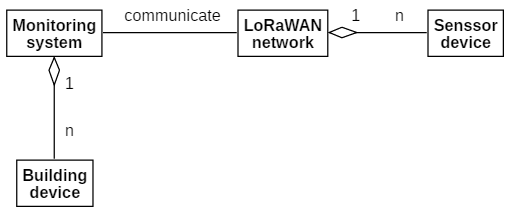
\includegraphics{figures/caseStudyB_high.png}
    \caption{High level architecture of the system}
    \label{fig:caseStudyAC}
\end{figure}
\\Designing the system with the aggregate computing is important to model the two different kind of entities and the communication network for the aggregate nodes.

\subsection*{Entities model}
The sensor devices are LoRa motes, so they are mapped in \mbox{\textit{Mote}} inside DingNet, while, according to \cref{sec:PoverD}, in the aggregate application they can be mapped in simple \mbox{\textit{ProtelisLoRaNode}}.
The building devices are not LoRa motes, so they do not require to be mapped in \mbox{\textit{ProtelisLoRaNode}} and they can be generic Protelis node.
Anyway it is decided to map them in \mbox{\textit{BuildingNode}}, which extends \mbox{\textit{ProtelisLoRaNode}}, \autoref{fig:caseBmodel_a}. This because:
\begin{itemize}
    \item the building node has not a physical mote then its topic will never receive a MQTT message; so it has not any overhead
    \item all the types of nodes have a base \mbox{\textit{ExecutionContext}} where introduce functions domain specific
    \item if in the future they will have a physical mote, it will not be necessary to change the system architecture.
\end{itemize}
\autoref{fig:caseBmodel_b} completes the model of the entities with their \mbox{\textit{ExecutionContext}}.
\mbox{\textit{SensorExecutionContext}} updates the knowledge-base of the node computing the CAQI index at each new sensed data received. It contains also all the methods for the logic domain specific. \mbox{\textit{BuildingExecutionContext}} extends it adding the capability to modify the temperature in its physical counterpart.
\begin{figure}[h]
    \centering
    \begin{subfigure}{.495\textwidth}
        \centering
        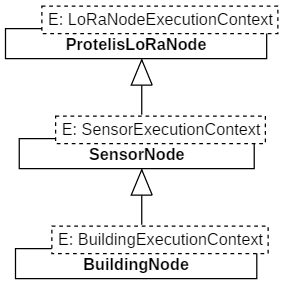
\includegraphics{figures/NodeAC_caseStudy.png}
        \caption{}
        \label{fig:caseBmodel_a}
    \end{subfigure}
    \begin{subfigure}{.495\textwidth}
        \centering
        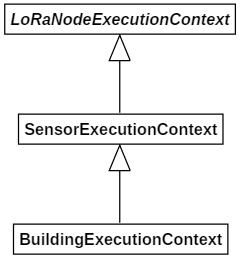
\includegraphics{figures/ECAC_caseStudy.png}
        \caption{}
        \label{fig:caseBmodel_b}
    \end{subfigure}
    \caption{Model of the aggregate entities.}
    \label{fig:caseBmodel}
\end{figure}
\subsection*{Interaction between Protelis nodes}
To complete the backend required from a Protelis application we need to:
\begin{enumerate}
    \item design and implement the communication between the Protelis node
    \item define the neighbourhood policy to define the neighbours of each node
\end{enumerate}
As neighbourhood policy it has been chosen a distance based policy. 
This policy has been chosen considering the application domain, in fact the behaviour of each node depends on the environment state in its area. 

\noindent To implement the \mbox{\textit{NetworkManager}} and enable the communication between Protelis nodes it has been chosen to use MQTT.
MQTT has been chosen because it is a lightweight protocol and enable devices to send the same message to more devices with only one communication.
This is very important in a large scale system where the nodes are displaced in many places and the connectivity can go down.

\noindent This system is composed also from mobile nodes and when one node change position its neighbours can change, as the neighbourhood of other nodes. 
So the definition of the neighbourhood cannot be done only at configuration time, but also after.
To do that it is defined the \mbox{\textit{NeighborhoodManager}}, which manage the neighbourhood of all the nodes.
It receives the update of the node position, recomputes the neighbourhoods, and communicates their to all the nodes. 
This entity allows also to modify the composition of the system at runtime adding or removing entities with all the neighbourhood updated automatically.

\section{Protelis program}
After presenting the design of the Protelis back-end, this section presents the Protelis program for the global behaviour of the system. 
The program, visible in \autoref{lst:program}, requires only 25 lines of code.
Methods \mbox{\textit{decreaseTemp}} and \mbox{\textit{increaseTemp}} modify the temperature of the building device of a delta temperature every half an hour.
These methods are build on top of the function \mbox{\textit{cyclicFunction}}, which is present in the developer API of the aggregate stack.
Lines 16 - 23 first create a computational field of sensed values and distances from the respective sensor. Then manipulate it to define a field of maximum temperature allowed for each device based on CAQI index.
The final part of the program defines the target temperature for each device and selects the correct method to achieve it. 

\lstinputlisting[
	float,
	language=Protelis,
	caption={Protelis program for monitoring application},
	label={lst:program},
]{listings/homeHeating_timer.pt}

\section{Simulation in DingNet}
This section presents the simulation of a possible scenario. 
The simulation is conducted over the city of Leuven with the DingNet simulator.
First, the setup of the simulated scenario is presented; then it will be discussed the simulation results in a qualitative way based on simulation snapshots.

\subsection{Setup}
The configuration of the simulation provides for a environment composed of the following entities:
\begin{itemize}
    \item 9 of the 11 DingNet network gateways (the others two are outside of the simulation region)
    \item 8 fixed sensors equipped with the PM10 sensor
    \item 2 mobile sensors equipped with PM10 and GPS sensors
    \item 3 building devices displaced in three different areas of the city.
\end{itemize}
All the sensors are configured to send a new measurement every hour, according to the specifications of the CAQI index for this polluting gas.
The low number of mobile sensors and building devices is only due to visualisation reasons. 

\subsection{Result}
\autoref{fig:simAC} shows three snapshots taken from a simulation run of five days.
The transparent layer represents the air quality level, that is obtained applying an inverse distance weighting on sensed values in the range of 1Km. 
Green color means ``very low'' level, while red color means ``high'' level.
The two motes with a red line are the mobile sensors, while the others are the fixed ones.
The building devices are represented with a black dot and a text with pattern ``X/Y/Z''.
% 
\begin{figure}[h]
    \centering
    \begin{tabular}{ll}
         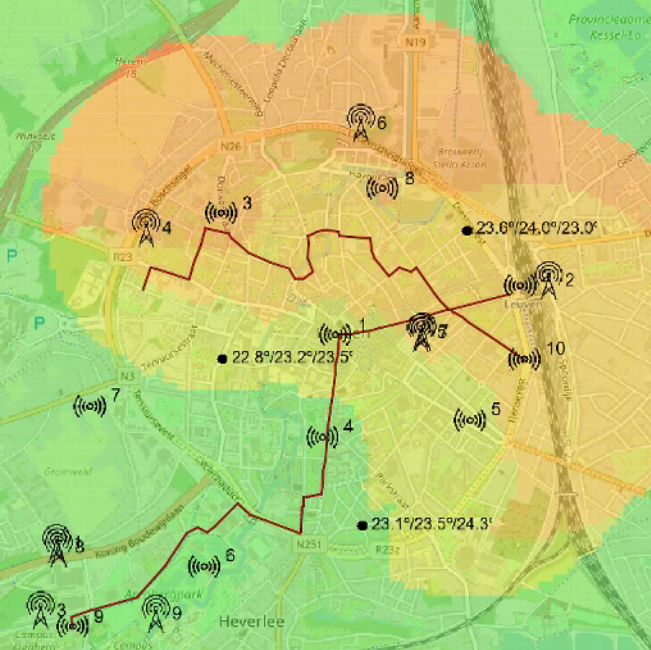
\includegraphics[scale=0.42]{figures/simACsnap1s.png}  &
         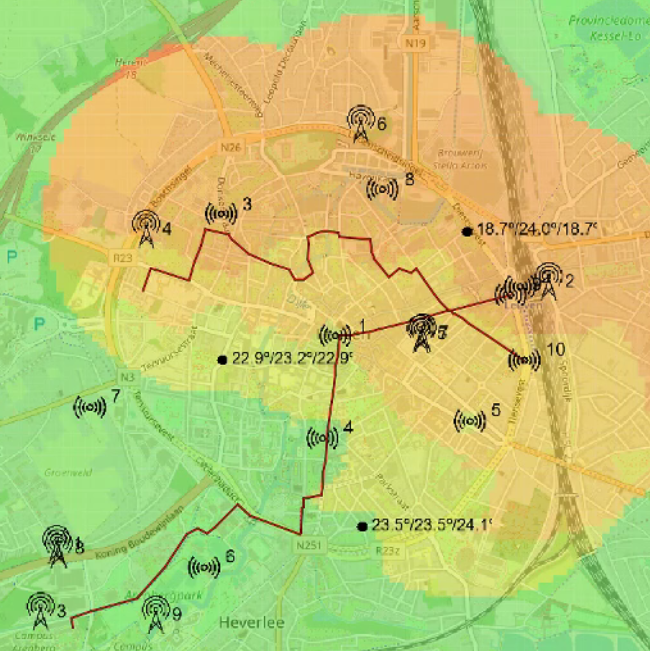
\includegraphics[scale=0.42]{figures/simACsnap2s.png}
    \end{tabular}
    \begin{tabular}{c}
         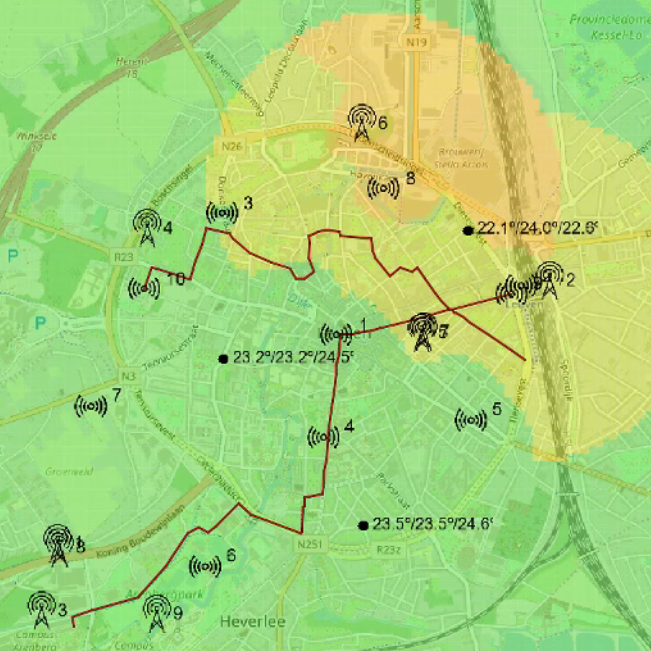
\includegraphics[scale=0.42]{figures/simACsnap3s.png} 
    \end{tabular}
    \caption{Three snapshots of a simulation run.}
    \label{fig:simAC}
\end{figure}
% 
X is its current temperature, Y is its desired temperature, and Z is its maximum reachable temperature based on pollution level.
The three snapshots show how the pollution changed during the five days of simulation, and how the building maximum reachable temperature is adapted consequently.
In particular the building in the north of the city has always the desired temperature greater then the maximum reachable. 
The building in the center of the city has first the desired temperature greater then the maximum reachable, but after the pollution change it is the opposite and the building reach its desired temperature.
Finally, the building in the south has always the desired temperature lower then the maximum reachable.

\paragraph{Concluding.} This chapter has presented a system designed with the aggregate computing paradigm over a LoRaWAN network, and simulated in the DingNet simulator.
After all the improvements and extensions on DingNet simulator, this case study has showed how it is possible simulate Protelis simulation in this platform. 
